\documentclass[10pt,twocolumn,letterpaper]{article}

% ---------- Fonts & Encoding ----------
\usepackage[utf8]{inputenc}
\usepackage[T1]{fontenc}
\usepackage[mono]{libertine}

% ---------- Page Layout ----------
\usepackage[margin=0.85in,columnsep=0.3in]{geometry}
\usepackage{parskip}
\setlength{\parskip}{4pt plus 1pt minus 1pt}

% ---------- Section Formatting ----------
\usepackage{titlesec}
\titleformat{\section}{\large\bfseries\sffamily}{\thesection}{0.8em}{}
\titleformat{\subsection}{\normalsize\bfseries\sffamily}{\thesubsection}{0.7em}{}
\titleformat{\subsubsection}{\normalsize\itshape\sffamily}{\thesubsubsection}{0.6em}{}
\titlespacing*{\section}{0pt}{14pt plus 2pt}{6pt plus 1pt}
\titlespacing*{\subsection}{0pt}{10pt plus 2pt}{4pt plus 1pt}
\titlespacing*{\subsubsection}{0pt}{8pt plus 2pt}{3pt plus 1pt}

% ---------- Math & Theorems ----------
\usepackage{amsmath}
\let\Bbbk\relax
\usepackage{amssymb}
\let\openbox\relax
\usepackage{amsthm}
\newtheorem{theorem}{Theorem}
\newtheorem{definition}{Definition}
\newtheorem{corollary}{Corollary}
\newtheorem{lemma}{Lemma}
\newtheorem{proposition}{Proposition}

% ---------- Tables ----------
\usepackage{booktabs}
\usepackage{tabularx}
\renewcommand{\arraystretch}{1.15}

% ---------- Figures & Graphics ----------
\usepackage{graphicx}
\usepackage{tikz}
\usetikzlibrary{positioning,arrows.meta,shapes.geometric,fit,backgrounds,calc}
\usepackage{caption}
\captionsetup{font=small,labelfont=bf,skip=6pt}

% ---------- Code Listings ----------
\usepackage{listings}
\usepackage{xcolor}
\definecolor{codebg}{HTML}{F7F7F8}
\definecolor{codeframe}{HTML}{E0E0E0}
\definecolor{kw}{HTML}{1A5276}
\definecolor{cmt}{HTML}{6C7A89}
\lstdefinestyle{code}{
    basicstyle=\ttfamily\footnotesize,
    breaklines=true,
    frame=single,
    framesep=6pt,
    xleftmargin=6pt,
    xrightmargin=2pt,
    backgroundcolor=\color{codebg},
    rulecolor=\color{codeframe},
    keywordstyle=\color{kw}\bfseries,
    commentstyle=\color{cmt}\itshape,
    numbers=none,
    captionpos=b,
    aboveskip=8pt,
    belowskip=8pt,
}
\lstset{style=code}

% ---------- Hyperlinks ----------
\usepackage[colorlinks=true,linkcolor=blue!50!black,citecolor=blue!50!black,urlcolor=blue!50!black]{hyperref}
\usepackage{url}
\usepackage{enumitem}

% ---------- Header ----------
\usepackage{fancyhdr}
\pagestyle{fancy}
\fancyhf{}
\renewcommand{\headrulewidth}{0.4pt}
\fancyhead[L]{\small\sffamily Private Distributed Inference on Consumer Hardware}
\fancyhead[R]{\small\sffamily\thepage}
\fancyfoot{}

% =====================================================================
\title{%
\vspace{-0.5cm}
{\LARGE\sffamily\bfseries Private Distributed Inference\\on Consumer Hardware}\\[8pt]
{\large\sffamily Enabling Confidential Computation on Third-Party Apple Silicon\\via Software Access Path Elimination}
}

\author{
    \textbf{Gajesh Naik} \\[4pt]
    {\small Eigen Labs} \\[2pt]
    {\small\texttt{gajesh@eigenlabs.org}}
}

\date{\small April 2026}

% =====================================================================
\begin{document}

\twocolumn[
\maketitle
\thispagestyle{fancy}

% ---------- Abstract ----------
\begin{@twocolumnfalse}
\begin{abstract}
\noindent
We present a system and method for private machine learning inference on a distributed network of consumer hardware. The core problem: a user wants to run an AI model on someone else's Mac, but the machine's owner---who has root access and physical custody---should not be able to see the user's prompts or the model's responses. The machines lack hardware Trusted Execution Environments (TEEs) for application-level memory isolation.

Our approach eliminates every software path through which inference data could be observed. The inference engine runs directly inside a single hardened Swift process---no subprocess, no local server, no inter-process communication---using \texttt{mlx-swift-lm} on the Apple Silicon GPU. The macOS kernel blocks all external access to this process's memory: debuggers are denied at the system call level (\texttt{PT\_DENY\_ATTACH}), memory-reading APIs are blocked by Hardened Runtime, and these protections cannot be disabled without rebooting, which terminates the process and erases its data. We prove that System Integrity Protection, once verified, is immutable for the process lifetime (Theorem~\ref{thm:sip}).

A multi-layer attestation architecture verifies each machine in the network: (1)~a Secure Enclave signature proves hardware-bound identity, (2)~Apple's MDM framework independently confirms the machine's security configuration, (3)~Apple's Managed Device Attestation (MDA) produces an Apple-signed certificate chain proving the device is genuine hardware, with an MDA nonce binding the provider's signing key to the attested device, (4)~periodic challenge-response confirms security posture has not degraded since enrollment, and (5)~APNs code-identity attestation proves the provider is running the genuine, team-signed Darkbloom binary by pushing an encrypted nonce that only a properly provisioned app can receive and requiring a Secure Enclave signature on the returned nonce.

After eliminating all software access paths, the only remaining attack requires physically probing the memory chips---which are soldered directly into Apple's System-on-Chip package. This is the same residual threat model accepted by Apple's Private Cloud Compute~\cite{apple-pcc} for Siri and Apple Intelligence. We validate the system end-to-end on production hardware with live inference, demonstrating negligible security overhead (12\,ms per request).
\end{abstract}
\vspace{16pt}
\end{@twocolumnfalse}
]

% =====================================================================
\section{Introduction}
\label{sec:intro}

When a user sends a prompt to a cloud AI service, that prompt travels to a server owned and operated by someone else. The user's privacy rests on a contractual promise---a privacy policy---not a technical guarantee. Hardware Trusted Execution Environments (TEEs) such as Intel TDX~\cite{intel-tdx}, AMD SEV-SNP~\cite{amd-sev}, and NVIDIA Confidential Computing~\cite{nvidia-cc} can provide cryptographic memory isolation, but these technologies exist only on enterprise server hardware costing \$14,000 or more.

Meanwhile, over 100 million Apple Silicon Macs have been sold since 2020. With 64--256\,GB of unified memory and 273--819\,GB/s memory bandwidth, they can run models with up to 235 billion parameters at interactive speeds. These machines sit idle most of the day. A distributed network that lets Mac owners contribute their idle compute for AI inference---while guaranteeing that they cannot see the prompts being processed---would make private inference available at a fraction of the cost of cloud TEEs.

The challenge is that Apple Silicon provides no hardware TEE accessible to third-party applications:

\begin{itemize}[leftmargin=*,itemsep=2pt,topsep=2pt]
    \item The \textbf{Secure Enclave} provides hardware-bound P-256 key generation and ECDSA signing, but cannot encrypt main system memory or provide isolated execution for arbitrary code.
    \item \textbf{App Attest} (\texttt{DCAppAttestService}) returns \texttt{false} for \texttt{isSupported} on macOS---it is available only on iOS and iPadOS. We therefore introduce APNs code-identity attestation as a macOS-compatible replacement for binary-identity proof (Section~\ref{sec:apns-attest}).
    \item No public API exposes boot measurements or PCR-style remote attestation.
\end{itemize}

We present a system that makes this possible. Rather than encrypting memory (which Apple Silicon cannot do for third-party code), we \emph{eliminate every software mechanism} through which the machine's owner could observe inference data---the same design philosophy Apple employs in Private Cloud Compute~\cite{apple-pcc}. Apple's PCC removes all software interfaces (shell, debugger, persistent storage) that could access inference data. We apply this principle to a harder problem: in PCC, Apple owns the hardware and controls physical access; in our system, the hardware owner is the adversary.

\textbf{Contributions.} This paper makes the following contributions:
\begin{enumerate}[leftmargin=*,itemsep=2pt,topsep=2pt]
    \item A \textbf{distributed private inference architecture} that enables confidential AI computation on a network of third-party Apple Silicon machines, where each machine's owner is assumed to be adversarial.
    \item A \textbf{formal security model} for this setting, including a proof that System Integrity Protection provides runtime immutability under standard assumptions (Theorem~\ref{thm:sip}), and a complete enumeration of the software attack surface.
    \item An \textbf{in-process inference design} that embeds the inference engine directly in a hardened Swift process using \texttt{mlx-swift-lm}, eliminating all inter-process communication channels that could be observed, with optional \textbf{hypervisor memory isolation} reported as telemetry for future RDMA hardening.
    \item A \textbf{multi-layer attestation architecture} combining Secure Enclave signatures, MDM-based independent verification, Apple MDA hardware attestation with Apple-signed certificate chains, MDA nonce-based SE key binding, periodic challenge-response with fresh security state, and APNs code-identity attestation proving the running binary is genuine.
    \item A \textbf{combined enrollment protocol} that unifies MDM enrollment and an ACME \texttt{device-attest-01} payload into a single configuration profile; the active hardware-provenance path today is MDA-over-MDM rather than ACME, with ACME retained for future transport-layer use.
    \item \textbf{End-to-end validation} on production hardware (Apple M2 and M4~Max) with live inference, demonstrating that the security mechanisms introduce negligible overhead.
    \item A \textbf{cost analysis} showing that Mixture-of-Experts models create 6--32$\times$ cost advantages on unified-memory hardware versus cloud GPUs, establishing economic feasibility.
\end{enumerate}

% =====================================================================
\section{Related Work}
\label{sec:related}

\textbf{Hardware TEE-based inference.}\quad Intel TDX~\cite{intel-tdx} and AMD SEV-SNP~\cite{amd-sev} encrypt VM memory and provide remote attestation. NVIDIA Confidential Computing~\cite{nvidia-cc} extends this to GPU memory. These approaches provide strong isolation but require enterprise server hardware. Our work achieves comparable privacy guarantees on consumer hardware without memory encryption.

\textbf{Distributed compute networks.}\quad Akash~\cite{akash} provides general compute with TEE support in development. io.net~\cite{ionet} aggregates GPU resources without hardware security guarantees. Ritual~\cite{ritual} uses zero-knowledge proofs and Intel SGX. Bittensor~\cite{bittensor} employs stake-weighted consensus for result verification. None address inference privacy on consumer hardware lacking TEEs.

\textbf{Apple Private Cloud Compute.}\quad PCC~\cite{apple-pcc} achieves inference privacy on Apple Silicon servers (M2~Ultra) without memory encryption through five requirements: stateless computation, enforceable guarantees, no privileged runtime access, non-targetability, and verifiable transparency. Implementation includes: no persistent storage, no SSH or shell access, immutable OS via Signed System Volume, cryptographic erasure on reboot, and OHTTP anonymization. Our work differs in that PCC operates in \emph{Apple-controlled data centers} with physical security (access controls, tamper detection), while our system must defend against the hardware owner as adversary.

\textbf{Cryptographic approaches.}\quad Fully Homomorphic Encryption~\cite{gentry-fhe} introduces $10^4$--$10^6\times$ computational overhead. Secure Multi-Party Computation~\cite{yao-mpc} requires multiple non-colluding servers. zkLLM~\cite{zkllm} and DeepProve-1~\cite{deepprove} verify inference integrity via zero-knowledge proofs but do not protect input privacy during computation. These remain impractical for interactive LLM inference at current performance levels.

% =====================================================================
\subsection{Comparison with Apple Private Cloud Compute}
\label{sec:pcc-comparison}

Table~\ref{tab:pcc} compares the system's security properties with Apple PCC.

\begin{table}[h]
\centering
\caption{Comparison with Apple Private Cloud Compute~\cite{apple-pcc}.}
\label{tab:pcc}
\vspace{4pt}
\small
\begin{tabularx}{\linewidth}{@{}l c X@{}}
\toprule
\textbf{Property} & \textbf{Apple PCC} & \textbf{This Work} \\
\midrule
Hardware owner & Trusted (Apple) & Adversarial \\
Physical security & Facility controls & Soldered LPDDR5x \\
Coordinator TEE & N/A (Apple infra) & AMD SEV-SNP \\
OS immutability & SSV & SIP + ARV + SSV hash \\
Shell/debug access & Removed entirely & Blocked at kernel level \\
Memory encryption & None & None \\
DMA/RDMA isolation & Facility controls & IOMMU default-deny; hypervisor Stage~2 planned \\
Provider verification & Apple-signed & SE + MDM + MDA + APNs code identity \\
Hardware provenance & Apple supply chain & Apple MDA certificates \\
Residual attack & Physical probing & Physical probing \\
\bottomrule
\end{tabularx}
\end{table}

The key distinction is who owns the hardware. In PCC, Apple owns the servers and controls physical access. In our system, the hardware belongs to an independent provider who may be adversarial. The multi-layer attestation architecture (Section~\ref{sec:attestation}) compensates for the absence of physical security by providing multiple independent verification paths, culminating in Apple-signed hardware provenance certificates. The result is that consumers get the same residual threat model---physical memory probing only---whether they use Apple's private cloud or our distributed network.

% =====================================================================
\section{Threat Model and Assumptions}
\label{sec:threat}

The fundamental challenge in distributed inference is that the person running the computation is not the person who owns the data. A provider contributes their Mac's compute, but should learn nothing about the prompts processed on it. This section formalizes what we assume about each party and what a malicious provider can attempt.

\subsection{Actors}

\begin{definition}[System Actors]
\label{def:actors}
We define four classes of actor:
\begin{itemize}[leftmargin=*,itemsep=1pt,topsep=2pt]
    \item $\mathcal{C}$ (Consumer): The party submitting inference requests. Trusted---they have no incentive to attack their own data.
    \item $\mathcal{K}$ (Coordinator): The routing and verification service. Trusted via hardware: runs in a Confidential VM (AMD SEV-SNP~\cite{amd-sev}) with cryptographic attestation of the deployed container image. The coordinator's memory is encrypted by the TEE hardware; neither the cloud operator nor the system operator can access it.
    \item $\mathcal{P}$ (Provider): The Mac owner contributing compute. \textbf{Assumed adversarial}---they own the hardware, have root access, and may actively attempt to read inference data. This is the strongest practical assumption: we guarantee privacy even if the provider is trying to break it.
    \item $\mathcal{A}$ (Apple): Trusted for the correctness of Secure Enclave hardware, SIP implementation, Kernel Integrity Protection, Hardened Runtime enforcement, IOMMU policy, code signature verification, and the Managed Device Attestation certificate authority.
\end{itemize}
\end{definition}

\subsection{Adversary Capabilities}

\begin{definition}[Threat Model]
\label{def:threat}
The adversarial provider $\mathcal{P}$ can:
\begin{itemize}[leftmargin=*,itemsep=1pt]
    \item Execute arbitrary code as root on the Mac
    \item Install any user-level software (subject to SIP restrictions)
    \item Reboot the machine at any time
    \item Physically access the machine exterior and ports
    \item Enable RDMA over Thunderbolt~5 (requires Recovery OS boot)
    \item Attempt to intercept or modify network traffic
\end{itemize}
The adversary $\mathcal{P}$ \emph{cannot}:
\begin{itemize}[leftmargin=*,itemsep=1pt]
    \item Exploit unpatched kernel vulnerabilities (Assumption~\ref{asm:kernel})
    \item Modify Secure Enclave firmware or extract its keys
    \item Desolder LPDDR5x memory from the SoC package without destroying it
    \item Compromise Apple's Managed Device Attestation signing infrastructure
\end{itemize}
\end{definition}

\begin{definition}[Assumptions]
\label{asm:kernel}
\textbf{Assumption 1} (Kernel Integrity): The macOS kernel has no unpatched vulnerabilities that allow SIP bypass, Hardened Runtime bypass, or KIP circumvention. Apple has patched all known SIP bypass CVEs (e.g., CVE-2022-22583, CVE-2022-42821, CVE-2023-32369) within weeks of disclosure.

\textbf{Assumption 2} (Secure Enclave Integrity): The Secure Enclave hardware and firmware correctly implement key generation, signing, and key isolation. This is analogous to trusting Intel SGX or ARM TrustZone hardware.

\textbf{Assumption 3} (Apple Attestation CA Integrity): Apple's Enterprise Attestation Root CA private key is not compromised, and Apple's attestation servers correctly verify device properties before issuing certificates. This is analogous to trusting any certificate authority in the Web PKI.
\end{definition}

\subsection{Security Goal}

In plain terms: a provider processes a prompt on their Mac, returns the result, and learns nothing about what the prompt said or what the model replied. More precisely:

\begin{definition}[Privacy Property]
\label{def:privacy}
Let $x$ be an inference input (prompt) and $y = f(x)$ the model output. The system satisfies the \emph{privacy property} if, for all polynomial-time adversaries $\mathcal{P}$:
\begin{equation}
\Pr[\mathcal{P} \text{ learns } x \text{ or } y] \leq \text{negl}(\lambda)
\end{equation}
where $\lambda$ is the security parameter, under Assumptions 1--3, excluding physical memory probing attacks requiring destructive hardware modification.
\end{definition}

% =====================================================================
\section{System Architecture}
\label{sec:arch}

The distributed network comprises three principal components: a \emph{coordinator} that routes consumer requests to providers and verifies their attestations, \emph{provider agents} running on Apple Silicon Macs that execute inference, and a \emph{Secure Enclave module} that gives each provider a hardware-bound cryptographic identity. The provider is a Swift CLI (\texttt{darkbloom}) that runs \texttt{mlx-swift-lm} in-process on the Apple Silicon GPU. Figure~\ref{fig:arch} depicts the complete architecture.

\begin{figure*}[t]
\centering
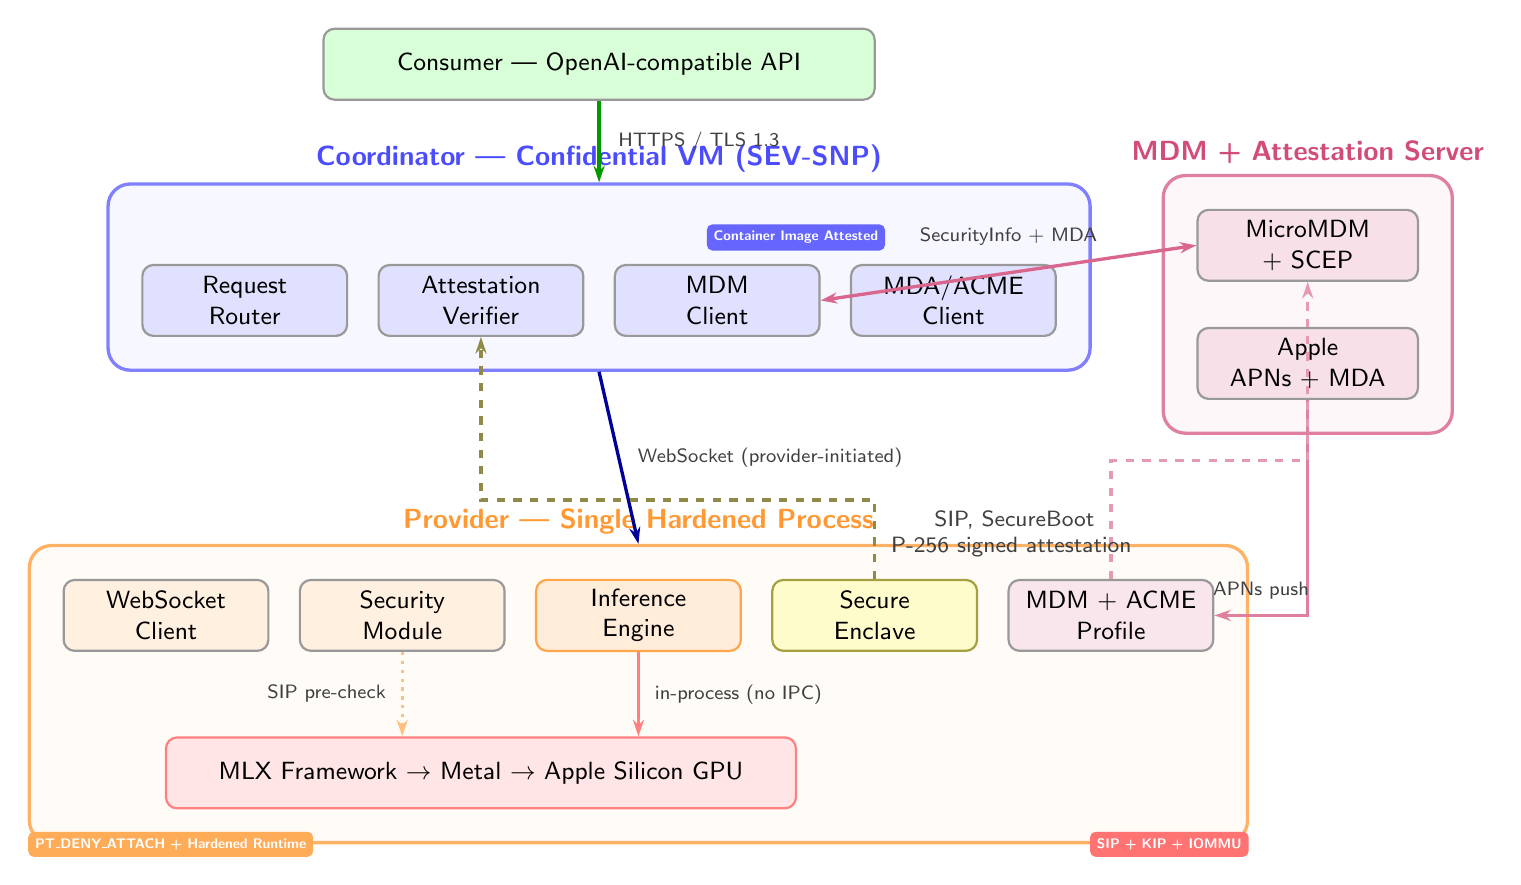
\begin{tikzpicture}[
    component/.style={draw=gray!80, thick, rounded corners=4pt, fill=#1, minimum width=2.6cm, minimum height=0.9cm, font=\small\sffamily, align=center},
    component/.default={white},
    groupbox/.style={draw=#1, very thick, rounded corners=8pt, inner sep=12pt},
    groupbox/.default={gray!50},
    arr/.style={-{Stealth[length=6pt,width=4pt]}, very thick, #1},
    arr/.default={gray!60},
    biarr/.style={{Stealth[length=6pt,width=4pt]}-{Stealth[length=6pt,width=4pt]}, very thick, #1},
    biarr/.default={gray!60},
    lbl/.style={font=\scriptsize\sffamily, #1},
    lbl/.default={gray!50!black},
    grouptitle/.style={font=\normalsize\sffamily\bfseries, #1},
    grouptitle/.default={black},
    badge/.style={font=\tiny\sffamily\bfseries, rounded corners=2pt, fill=#1, text=white, inner sep=2.5pt},
]

\node[component=green!15, minimum width=7cm] (consumer) at (0, 0) {Consumer --- OpenAI-compatible API};

\node[component=blue!12] (router) at (-4.5, -3) {Request\\Router};
\node[component=blue!12] (attverify) at (-1.5, -3) {Attestation\\Verifier};
\node[component=blue!12] (mdmclient) at (1.5, -3) {MDM\\Client};
\node[component=blue!12] (acmeca) at (4.5, -3) {MDA/ACME\\Client};
\node[minimum height=0.5cm, minimum width=1cm] (coordspacer) at (4.5, -2.2) {};
\begin{scope}[on background layer]
\node[groupbox=blue!50, fill=blue!3, fit=(router)(attverify)(mdmclient)(acmeca)(coordspacer),
      label={[grouptitle=blue!70]above:{Coordinator --- Confidential VM (SEV-SNP)}}] (coordbox) {};
\end{scope}
\node[badge=blue!60] at (2.5, -2.2) {Container Image Attested};

\node[component=purple!12, minimum width=2.8cm] (mdmserver) at (9, -2.3) {MicroMDM\\+ SCEP};
\node[component=purple!12, minimum width=2.8cm] (apns) at (9, -3.8) {Apple\\APNs + MDA};
\begin{scope}[on background layer]
\node[groupbox=purple!50, fill=purple!3, fit=(mdmserver)(apns),
      label={[grouptitle=purple!70]above:{MDM + Attestation Server}}] (mdmbox) {};
\end{scope}

\node[component=orange!12] (wsclient) at (-5.5, -7) {WebSocket\\Client};
\node[component=orange!12] (secmod) at (-2.5, -7) {Security\\Module};
\node[component=orange!15, draw=orange!70] (infereng) at (0.5, -7) {Inference\\Engine};
\node[component=yellow!20, draw=yellow!60!black] (secenclave) at (3.5, -7) {Secure\\Enclave};
\node[component=red!10, draw=red!50, minimum width=8cm, minimum height=0.9cm]
    (mlxgpu) at (-1.5, -9) {MLX Framework $\to$ Metal $\to$ Apple Silicon GPU};
\node[component=purple!10] (mdmprof) at (6.5, -7) {MDM + ACME\\Profile};
\begin{scope}[on background layer]
\node[groupbox=orange!60, fill=orange!3, fit=(wsclient)(secmod)(infereng)(secenclave)(mlxgpu)(mdmprof),
      label={[grouptitle=orange!80]above:{Provider --- Single Hardened Process}}] (provbox) {};
\end{scope}
\node[badge=orange!65, anchor=west] at (provbox.south west) {PT\_DENY\_ATTACH + Hardened Runtime};
\node[badge=red!55, anchor=east] at (provbox.south east) {SIP + KIP + IOMMU};

% ===== ARROWS =====
\draw[arr=green!60!black] (consumer.south) -- (coordbox.north) node[lbl, midway, right=3pt] {HTTPS / TLS 1.3};
\draw[arr=blue!60!black] (coordbox.south) -- (provbox.north) node[lbl, midway, right=3pt] {WebSocket (provider-initiated)};
\draw[biarr=purple!60] (mdmclient.east) -- (mdmserver.west) node[lbl, midway, above=6pt] {SecurityInfo + MDA};
\draw[arr=purple!50] (apns.south) |- (mdmprof.east) node[lbl, pos=0.75, above=2pt] {APNs push};
\draw[arr=purple!40, dashed] (mdmprof.north) -- ++(0, 1.5) node[lbl, left=2pt, pos=0.5] {\footnotesize SIP, SecureBoot} -| (mdmserver.south);
\draw[arr=yellow!50!black, dashed] (secenclave.north) -- ++(0, 1.0) node[lbl, right=2pt, pos=0.4] {\footnotesize P-256 signed attestation} -| (attverify.south);
\draw[arr=red!50] (infereng.south) -- (mlxgpu.north-|infereng.south) node[lbl, midway, right=2pt] {in-process (no IPC)};
\draw[arr=orange!50, dotted] (secmod.south) -- (mlxgpu.north-|secmod.south) node[lbl, midway, left=2pt] {SIP pre-check};

\end{tikzpicture}
\caption{System architecture. The consumer connects via HTTPS (optionally NaCl Box sealed) to a coordinator running in a Confidential VM. The coordinator routes requests to provider Macs over provider-initiated WebSocket connections, re-encrypting each request with a per-request NaCl Box to the provider's attested X25519 key. Each provider runs inference in a single hardened Swift process protected by PT\_DENY\_ATTACH, Hardened Runtime, SIP, KIP, and IOMMU. The Secure Enclave provides hardware-bound P-256 identity; APNs code-identity attestation proves the binary is genuine. MDA-over-MDM (not ACME) is the operative hardware-provenance path today.}
\label{fig:arch}
\end{figure*}

\subsection{In-Process Inference}
\label{sec:inprocess}

Traditional inference serving architectures (vLLM, Ollama, llama.cpp) run the engine as a separate HTTP server process. This creates two attack surfaces: (a)~localhost TCP traffic can be captured via \texttt{tcpdump}, which functions even with SIP enabled; and (b)~the subprocess binary can be replaced with a version that logs requests.

Our architecture eliminates both attack surfaces by embedding the inference engine directly in a single hardened Swift process. The provider uses \texttt{mlx-swift-lm} (a fork maintained under \texttt{libs/mlx-swift-lm}) to load model weights and run generation inside the same address space that holds the WebSocket client, attestation signer, and encryption keys:

\begin{lstlisting}[language=Swift,caption={Inference executes inside the hardened Swift process address space. No subprocess, HTTP server, socket, or pipe is created.}]
import MLXLMCommon

// Model loaded in-process
let container = try await LLMModelFactory.shared.loadContainer(
    configuration: config)

// Inference in protected memory
let result = try await container.perform { _, tokenizer in
    try generate(promptTokens: tokens,
                 parameters: params,
                 model: $0)
}
\end{lstlisting}

Model weights (up to 76\,GB for a 122B-parameter model at 4-bit quantization), tokenizer, and all intermediate activations reside in a single process address space. This space is protected by three kernel-enforced mechanisms described in Section~\ref{sec:access-path}. Because the Swift binary is code-signed and SIP prevents execution of modified signed binaries, the only binaries that can act as decryption endpoints are the genuine team-signed build (further proved by APNs code-identity attestation, Section~\ref{sec:apns-attest}) and any blessed variants tracked in a transparency log.

\subsubsection{Memory Sanitization}

After each inference request completes, buffers containing prompts and model outputs are zeroed using \texttt{memset\_s}, which is guaranteed not to be optimized away by the compiler, ensuring sensitive data is overwritten before the buffers are released.

\subsection{Access Path Elimination}
\label{sec:access-path}

Three kernel-enforced mechanisms jointly eliminate all software paths to the inference process's memory:

\begin{enumerate}[leftmargin=*,itemsep=2pt,topsep=2pt]
    \item \textbf{\texttt{PT\_DENY\_ATTACH}} (ptrace constant 31): Invoked at process startup before any sensitive data is loaded. Instructs the macOS kernel to permanently deny all \texttt{ptrace} requests against this process, including from root. This blocks \texttt{lldb}, \texttt{dtrace}, and Instruments.

    \item \textbf{Hardened Runtime}: The binary is code-signed with hardened runtime options and explicitly \emph{without} the \texttt{com.apple.security.get-task-allow} entitlement. The kernel denies \texttt{task\_for\_pid()} and \texttt{mach\_vm\_read()} from any external process.

    \item \textbf{System Integrity Protection (SIP)}: Enforces both of the above at the kernel level. With SIP enabled, root cannot circumvent Hardened Runtime protections, load unsigned kernel extensions, or modify protected system binaries. Section~\ref{sec:sip} proves that SIP, once verified, is immutable for the process lifetime.
\end{enumerate}

\subsection{Coordinator Trust Boundary}

The coordinator runs in a Confidential VM (AMD SEV-SNP) on cloud infrastructure. The container image is cryptographically attested---consumers can verify that the coordinator executes unmodified code. The coordinator's memory is encrypted by the TEE hardware; neither the cloud infrastructure operator nor the system operator can access it.

The coordinator performs request routing, attestation verification, billing, and key management. Consumers may optionally seal requests to the coordinator's long-lived X25519 key; in all cases the coordinator decrypts the request body inside its Confidential-VM memory for routing and billing. Prompt content is never logged or retained, and is immediately re-encrypted with a fresh per-request NaCl Box to the selected provider's attested X25519 key (Section~\ref{sec:e2e}). The coordinator is therefore a trusted plaintext intermediary for routing, not a blind relay.

% =====================================================================
\section{End-to-End Encryption}
\label{sec:e2e}

Encryption is hop-by-hop rather than strictly end-to-end. The system uses NaCl Box (X25519 key agreement + XSalsa20-Poly1305 authenticated encryption)~\cite{nacl} for both legs.

\subsection{Two-Leg Model}

\textbf{Consumer $\rightarrow$ coordinator.} By default the consumer sends plaintext over TLS. Optionally, the consumer may seal the request body to the coordinator's long-lived X25519 public key (advertised at \texttt{GET /v1/encryption-key}). The coordinator decrypts the body inside its Confidential-VM memory for routing and billing.

\textbf{Coordinator $\rightarrow$ provider.} For every inference request the coordinator:
\begin{enumerate}[leftmargin=*,itemsep=1pt]
    \item Generates an ephemeral X25519 key pair $(sk_e, pk_e)$
    \item Generates a random 24-byte nonce $n$
    \item Computes the shared secret and encrypts the request body: $c = \text{Box}(m, n, pk_{\text{provider}}, sk_e)$
    \item Sends $(pk_e, n \| c)$ to the provider over the outbound WebSocket
\end{enumerate}

The provider decrypts using its in-memory X25519 key $K$ (bound to its Secure Enclave identity via the attestation blob, Section~\ref{sec:se-attest}). Response SSE chunks are encrypted back to the coordinator's ephemeral public key and decrypted by the coordinator before being relayed to the consumer (re-sealed if consumer sealing is enabled).

\subsection{Forward Secrecy}

Each request uses a fresh coordinator ephemeral key pair. Compromise of any single ephemeral key does not enable decryption of past or future requests. The provider's X25519 key $K$ lives only in the hardened process's protected memory; its binding to the Secure Enclave identity is verified by the coordinator.

% =====================================================================
\section{Five-Layer Attestation Architecture}
\label{sec:attestation}

The attestation architecture provides five independent layers of verification, each addressing distinct threat vectors. Table~\ref{tab:trust-layers} summarizes the layers and their properties.

\begin{table}[h]
\centering
\caption{Five-layer attestation architecture. Each layer addresses threats not covered by the others.}
\label{tab:trust-layers}
\vspace{4pt}
\scriptsize
\begin{tabular}{@{}clp{2.8cm}@{}}
\toprule
\textbf{Layer} & \textbf{Mechanism} & \textbf{Threat Addressed} \\
\midrule
1 & SE P-256 ECDSA & Hardware-bound identity; replay prevention \\
2 & MDM SecurityInfo & Independent SIP/SecureBoot verification \\
3 & MDA-over-MDM & Apple-signed hardware provenance \\
4 & Challenge-response & Liveness; continuous security state \\
5 & APNs code identity & Genuine binary proof (v0.6.0) \\
\bottomrule
\end{tabular}
\end{table}

\subsection{Layer 1: Secure Enclave Attestation}
\label{sec:se-attest}

On first execution, the provider generates a P-256 ECDSA signing key inside Apple's Secure Enclave via CryptoKit. The private key never leaves the Secure Enclave hardware---the \texttt{dataRepresentation} stored on disk is an opaque handle that functions only on the device that created it. The provider constructs a signed attestation blob:

\begin{table}[h]
\centering
\caption{Attestation blob fields. JSON-encoded with deterministic key ordering (alphabetical) and signed by the Secure Enclave P-256 key.}
\vspace{4pt}
\scriptsize
\begin{tabular}{@{}llp{3.0cm}@{}}
\toprule
\textbf{Field} & \textbf{Type} & \textbf{Purpose} \\
\midrule
\texttt{authenticatedRootEnabled} & bool & Sealed system volume (ARV) \\
\texttt{binaryHash} & hex string & SHA-256 of running binary \\
\texttt{chipName} & string & Hardware identity \\
\texttt{encryptionPublicKey} & base64 & X25519 key bound to this identity \\
\texttt{hardwareModel} & string & Machine model identifier \\
\texttt{hypervisorActive} & bool & Hypervisor VM active (Section~\ref{sec:hypervisor}) \\
\texttt{osVersion} & string & macOS version \\
\texttt{publicKey} & base64 & P-256 public key (raw X$\|$Y) \\
\texttt{rdmaDisabled} & bool & RDMA status via \texttt{rdma\_ctl} \\
\texttt{secureBootEnabled} & bool & Secure Boot status \\
\texttt{secureEnclaveAvailable} & bool & SE hardware present \\
\texttt{serialNumber} & string & Device serial for MDM cross-ref \\
\texttt{sipEnabled} & bool & SIP status \\
\texttt{systemVolumeHash} & hex string & APFS snapshot hash \\
\texttt{timestamp} & ISO 8601 & Freshness \\
\bottomrule
\end{tabular}
\end{table}

Three fields merit particular attention:

\textbf{serialNumber.}\quad The hardware serial number enables the coordinator to correlate the device with its MDM enrollment record and request independent security verification. This field bridges Layer~1 (self-reported) to Layers~2 and~3 (independently verified).

\textbf{binaryHash.}\quad The SHA-256 hash of the running provider binary. Because this value is self-reported by the measurer---the potentially adversarial provider---it cannot serve as a standalone trust signal: a modified binary can simply report the hash of a blessed version. Starting in v0.6.0, \texttt{binaryHash} is used only for drift telemetry and transparency-log matching; the active code-identity proof is APNs code-identity attestation (Section~\ref{sec:apns-attest}). The hash is retained in the SE-signed status canonical so that a blessed-build policy can be re-enabled as a rollback or emergency gate.

\textbf{encryptionPublicKey.}\quad Binds the provider's X25519 encryption key (used for hop-by-hop encrypted inference, Section~\ref{sec:e2e}) to the same Secure Enclave identity. The coordinator verifies this matches the key in the registration message, proving the same physical device controls both the signing and decryption keys.

\subsubsection{Cross-Language Signature Verification}

The attestation protocol spans two programming languages: Swift (Secure Enclave signing and provider agent) and Go (coordinator verification). Both must produce byte-identical JSON representations for signature verification to succeed. We enforce this through:
\begin{itemize}[leftmargin=*,itemsep=1pt]
    \item Struct fields declared in alphabetical order (by JSON key name) in both languages
    \item Swift's \texttt{JSONEncoder} configured with \texttt{.sortedKeys} output formatting
    \item Go coordinator preserves raw attestation bytes (\texttt{json.RawMessage}) for verification, with a \texttt{marshalSortedJSON} fallback using \texttt{map[string]interface\{\}} (Go 1.12+ marshals map keys in sorted order)
    \item \texttt{omitempty} handling: nil fields omitted (not set to null)
    \item ISO 8601 timestamp format with consistent precision
    \item Base64 standard alphabet (no URL-safe variant); raw P-256 key format (64 bytes: X$\|$Y, no 0x04 prefix)
\end{itemize}

\subsubsection{Coordinator Verification Procedure}

The coordinator verifies each attestation through the following steps:
\begin{enumerate}[leftmargin=*,itemsep=1pt]
    \item Decode the P-256 public key from the attestation blob (64-byte raw X$\|$Y format)
    \item Hash the original JSON blob bytes with SHA-256
    \item Verify the DER-encoded ECDSA signature against the hash
    \item Enforce: \texttt{secureEnclaveAvailable} = true, \texttt{sipEnabled} = true, \texttt{secureBootEnabled} = true
    \item Verify: \texttt{encryptionPublicKey} matches the registration message
    \item Verify: \texttt{timestamp} is within acceptable freshness window
    \item Record \texttt{binaryHash} for drift telemetry and transparency-log matching
    \item If all pass, proceed to Layer~2 verification
\end{enumerate}

\subsection{Layer 2: MDM-Based Independent Verification}
\label{sec:mdm}

Secure Enclave attestation (Layer~1) has two inherent limitations: (a)~the coordinator cannot prove the P-256 signing key resides in the Secure Enclave rather than in software, since both produce identical ECDSA signatures; and (b)~the SIP status in the attestation blob is obtained via \texttt{csrutil status}, a software check that could theoretically be spoofed on a compromised system.

Layer~2 addresses both limitations through \emph{independent verification}: the coordinator queries the device's security posture through Apple's MDM framework, which returns data from the OS MDM subsystem---not from the provider software.

\subsubsection{SecurityInfo Command}

Apple's MDM \texttt{SecurityInfo} command~\cite{apple-mdm} returns the following fields, as reported by the operating system's MDM client:

\begin{table}[h]
\centering
\caption{Fields returned by the MDM \texttt{SecurityInfo} command. The coordinator requires SIP enabled, Secure Boot ``full,'' and Authenticated Root Volume enabled.}
\vspace{4pt}
\small
\begin{tabular}{@{}lp{4.2cm}@{}}
\toprule
\textbf{Field} & \textbf{Verification Purpose} \\
\midrule
\texttt{SIPEnabled} & SIP active---root cannot modify \texttt{/System} or bypass Hardened Runtime \\
\texttt{SecureBootLevel} & ``full'': only Apple-signed code at boot \\
\texttt{AuthRootVolume} & Signed System Volume Merkle tree intact \\
\texttt{FDE\_Enabled} & FileVault disk encryption active \\
\texttt{RecoveryLock} & Recovery Mode requires password \\
\texttt{FirewallEnabled} & Application firewall active \\
\bottomrule
\end{tabular}
\end{table}

The coordinator cross-checks these values against the self-reported attestation blob. Any discrepancy results in immediate rejection.

\subsubsection{Authenticated Root Volume}
\label{sec:arv}

The Authenticated Root Volume (ARV) seals the macOS system volume with a Merkle tree of SHA-256 hashes. Any modification to any system file---including \texttt{mdmclient}, \texttt{csrutil}, and kernel caches---breaks the seal and prevents the volume from mounting. ARV provides a stronger guarantee than SIP alone: SIP prevents \emph{runtime} modifications, while ARV proves the \emph{entire system volume} is Apple's unmodified build.

The \texttt{systemVolumeHash} field in the attestation blob contains the cryptographic hash of the APFS system volume snapshot, uniquely identifying the exact macOS build. The coordinator can cross-reference this against known-good builds published by Apple.

\subsection{Layer 3: MDA-over-MDM Hardware Attestation}
\label{sec:mda}

Layers~1 and~2 verify security \emph{posture} (is SIP enabled?) but do not provide cryptographic proof of hardware \emph{identity} (is this a genuine Apple device?). Layer~3 addresses this through Apple's Managed Device Attestation (MDA) protocol, requested over MDM via the \texttt{DeviceInformation} command with \texttt{DevicePropertiesAttestation}~\cite{apple-mda}.

\subsubsection{Protocol Overview}

After the device enrolls in MDM, the coordinator sends a \texttt{DeviceInformation} command requesting \texttt{DevicePropertiesAttestation}. The device contacts Apple's attestation servers and returns a DER-encoded X.509 certificate chain:
\begin{itemize}[leftmargin=*,itemsep=0pt]
    \item \textbf{Leaf}: Device certificate with Apple-assigned OIDs encoding hardware properties
    \item \textbf{Intermediate}: Apple Enterprise Attestation Sub CA~1 (P-384)
    \item \textbf{Root}: Apple Enterprise Attestation Root CA (P-384, valid until 2047)
\end{itemize}

The coordinator verifies the chain against the embedded Apple Enterprise Attestation Root CA, extracts the OID-encoded properties, and cross-checks the serial number against the provider's self-reported attestation. The complete certificate chain is stored and exposed via a public API endpoint, enabling consumers to independently verify each provider against Apple's publicly available root CA certificate.

\subsubsection{Certificate OID Fields}

The leaf certificate in Apple's attestation chain encodes device properties as X.509 extensions with Apple-assigned OIDs:

\begin{table}[h]
\centering
\caption{Apple-assigned OIDs in MDA leaf certificates. These values are signed by Apple's Enterprise Attestation Root CA and cannot be forged.}
\vspace{4pt}
\scriptsize
\begin{tabular}{@{}lll@{}}
\toprule
\textbf{OID Suffix} & \textbf{Property} & \textbf{Verification Use} \\
\midrule
100.8.9.1 & Serial Number & Device identity \\
100.8.9.2 & UDID & Device identity \\
100.8.10.1 & OS Version & OS currency \\
100.8.10.2 & SepOS Version & SE firmware version \\
100.8.10.3 & LLB Version & Boot chain integrity \\
100.8.11.1 & Freshness Code & Replay prevention / SE key binding \\
100.8.13.1 & SIP Status & SIP independently verified \\
100.8.13.2 & Secure Boot & Boot security level \\
100.8.13.3 & Kext Status & Kernel extension policy \\
\bottomrule
\multicolumn{3}{@{}l}{\scriptsize All OIDs prefixed with 1.2.840.113635.}
\end{tabular}
\end{table}

\subsubsection{SE Key Binding via Freshness Nonce}

When requesting MDA, the coordinator supplies a \texttt{DeviceAttestationNonce} equal to SHA-256 of the provider's SE public key. Apple embeds that hash in the \texttt{FreshnessCode} OID of the signed leaf certificate. The coordinator verifies that the returned freshness code matches the hash of the SE public key it already accepted, cryptographically binding the SE signing key to Apple-attested genuine hardware.

\subsubsection{ACME \texttt{device-attest-01} Limitations}

The enrollment profile still contains an ACME \texttt{device-attest-01} payload, but it is \emph{not} the operative production trust anchor today. Hardware-bound ACME identities on macOS land in the data-protection keychain inside a restricted system access group that is inaccessible to third-party applications, including the Darkbloom provider; only Apple system services such as Wi-Fi EAP-TLS and Safari mTLS can use them. In addition, the ACME leaf issued by our setup does not currently carry the SIP/SecureBoot OIDs, and the mTLS ingress path that would populate the verifying headers is not functional in production. Consequently, the active hardware-provenance path is MDA-over-MDM, with ACME retained for future transport-layer use.

\subsubsection{Comparison with SecurityInfo}

Table~\ref{tab:secinfo-vs-mda} compares the two independent verification mechanisms.

\begin{table}[h]
\centering
\caption{MDM SecurityInfo (Layer~2) vs.\ MDA-over-MDM (Layer~3).}
\vspace{4pt}
\small
\begin{tabular}{@{}lcc@{}}
\toprule
\textbf{Property} & \textbf{SecurityInfo} & \textbf{MDA} \\
\midrule
Trust anchor & OS MDM client & Apple Root CA \\
Forgery requires & SIP disabled & Apple CA compromise \\
Proves identity & No & Yes (serial, UDID) \\
Proves security & Yes (SIP, boot) & Yes (SIP, boot, SepOS) \\
Latency & Seconds & Minutes (Apple servers) \\
Availability & Always & Requires MDM enrollment \\
\bottomrule
\end{tabular}
\label{tab:secinfo-vs-mda}
\end{table}

\subsection{Layer 4: Continuous Challenge-Response}
\label{sec:challenge}

Layers~1--3 establish trust at enrollment time. Layer~4 provides continuous assurance that the provider's security posture has not changed since enrollment.

Every 5 minutes, the coordinator generates a random 32-byte nonce $n$ and timestamp $t$, and sends an \texttt{attestation\_challenge} message to the provider. The provider must:

\begin{enumerate}[leftmargin=*,itemsep=1pt]
    \item Check current SIP status via \texttt{csrutil status}
    \item Check current Secure Boot status
    \item Check current RDMA status via \texttt{rdma\_ctl status}
    \item Check current hypervisor status
    \item Compute signature $\sigma = \text{Sign}_{\text{SE}}(n \| t \| \text{pk})$ where $\text{pk}$ is the registered public key
    \item Return $(\sigma, n, \text{pk}, \text{sip\_enabled}, \text{secure\_boot\_enabled}, \text{rdma\_disabled}, \text{hypervisor\_active})$ within 30 seconds
\end{enumerate}

The coordinator verifies:
\begin{itemize}[leftmargin=*,itemsep=1pt]
    \item Nonce $n$ matches the sent value
    \item Public key $\text{pk}$ matches the registered key
    \item ECDSA signature $\sigma$ is valid
    \item \texttt{sip\_enabled} = true (immediate untrust if false)
    \item \texttt{secure\_boot\_enabled} = true (immediate untrust if false)
    \item Records \texttt{rdma\_disabled} and \texttt{hypervisor\_active} for telemetry and future policy enforcement
\end{itemize}

\textbf{Immediate untrust policy:} If SIP or Secure Boot is reported as disabled, the provider is immediately marked untrusted with no grace period. Disabled SIP or Secure Boot indicates a deliberate reboot with weakened security (by Theorem~\ref{thm:sip}, SIP cannot be disabled without rebooting). RDMA status and hypervisor activity are currently reported as telemetry; strict RDMA-without-hypervisor routing enforcement is reserved for future deployment.

\textbf{Failure escalation:} Three consecutive signature verification failures result in untrust marking. This catches providers experiencing connectivity issues versus providers that have been replaced or compromised.

\textbf{Reconnection scenario:} If a provider reboots (e.g., to disable SIP), disconnects, and reconnects, the reconnection triggers a fresh registration with a new attestation blob. If the new attestation reports SIP as disabled, the provider is rejected. If the provider lies about SIP status, the next MDM SecurityInfo query independently reveals the true state.

\subsection{Layer 5: APNs Code-Identity Attestation}
\label{sec:apns-attest}

Layers~1--4 establish hardware identity and continuous security posture, but they do not prove \emph{which binary} is running on the device. A malicious provider could run a fork that logs prompts while presenting a valid SE key and MDA certificate. Layer~5 closes this gap through APNs code-identity attestation (v0.6.0).

This is a practical breakthrough because macOS does not expose \texttt{DCAppAttestService} to third-party apps---\texttt{isSupported} returns \texttt{false} on macOS---so App Attest cannot be used to prove binary identity. A self-reported \texttt{binaryHash} is equally insufficient, because the measurer is the potentially adversarial provider. APNs code-identity attestation solves the problem without a new Apple API: it repurposes Apple's existing push-delivery infrastructure as a non-self-reportable code-identity oracle.

\textbf{Why APNs proves code identity.} Only a process that satisfies three conditions can receive a push for our topic \texttt{io.darkbloom.provider}:
\begin{enumerate}[leftmargin=*,itemsep=1pt]
    \item It is signed with our Developer ID team certificate.
    \item It carries our globally unique App ID \texttt{io.darkbloom.provider}.
    \item It is authorized by an Apple-signed provisioning profile containing the \texttt{aps-environment} entitlement.
\end{enumerate}
These conditions are enforced at launch by the \texttt{AppleMobileFileIntegrity.kext} kernel extension (AMFI) working with the user-space \texttt{amfid} daemon. AMFI validates the code signature, entitlements, and provisioning profile before the process is allowed to register for remote notifications with Apple's push service. A modified binary, a re-signed binary under a different Team ID, or an app lacking the entitlement cannot obtain a valid APNs device token for our topic. This makes APNs delivery a strong, Apple-mediated statement that the receiving process is the genuine Darkbloom build.

\textbf{Protocol.} At registration the provider sends its APNs device token $T$ alongside its X25519 public key $K$ and SE public key. The coordinator:
\begin{enumerate}[leftmargin=*,itemsep=1pt]
    \item Binds $T \leftrightarrow K$ to the WebSocket connection.
    \item Generates a fresh 32-byte nonce $n$.
    \item Encrypts the nonce to $K$ using NaCl Box: $c = \text{Box}(n, K)$.
    \item Sends an APNs background push to $T$ carrying $c$.
\end{enumerate}

Only the genuine Darkbloom binary receives the push. It decrypts $n$ with $K$, signs the nonce with its SE P-256 key, and returns $(n, \sigma)$ over the same WebSocket. The coordinator verifies:
\begin{itemize}[leftmargin=*,itemsep=1pt]
    \item The returned nonce matches the one it pushed.
    \item The SE signature $\sigma$ is valid against the public key bound at registration.
\end{itemize}

On success the connection is marked \texttt{CodeAttested}. Private text routing requires this flag once the code-attestation enforcement deadline has passed. The flag is per-connection and in-memory; reconnecting forces re-attestation, because a SIP downgrade requires a reboot which drops the WebSocket.

\begin{figure}[ht]
\centering
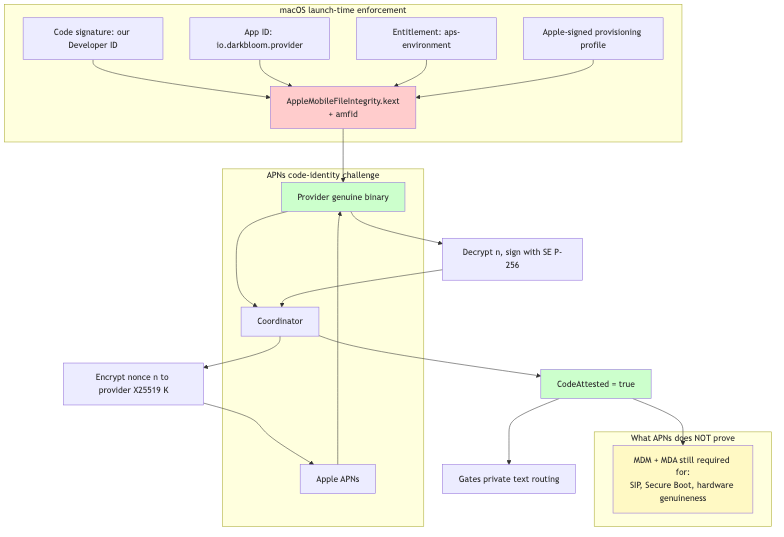
\includegraphics[width=\columnwidth]{../docs/assets/diagrams/apns-code-identity.png}
\caption{APNs code-identity attestation. AMFI (\texttt{AppleMobileFileIntegrity.kext}) enforces code signature, App ID, and \texttt{aps-environment} entitlement at launch, so only the genuine Darkbloom binary can register for our push topic. The coordinator pushes an encrypted nonce to that topic; the provider decrypts it with its bound X25519 key and returns a Secure Enclave signature, proving the WebSocket session is backed by genuine code holding the decryption key. MDM and MDA remain required for SIP, Secure Boot, and hardware provenance.}
\label{fig:apns}
\end{figure}

\textbf{MDM remains required.} APNs code identity proves \emph{which binary} is running, but it does not prove the device's security posture (SIP, Secure Boot, hardware genuineness). Those properties still require Layer~2 (MDM \texttt{SecurityInfo}) and Layer~3 (MDA-over-MDM). The provider must therefore still install the combined MDM enrollment profile; APNs is not a replacement for MDM, but rather the missing code-identity piece that MDM and MDA do not provide.

\textbf{Limits.} Background push delivery is best-effort and device-budget-throttled; the coordinator can switch to alert mode if reliability becomes an issue. APNs requires a logged-in macOS GUI Aqua session, so headless or login-screen Macs cannot become code-attested and fail closed for private traffic. APNs binds App ID/Team ID, not exact binary version; version/downgrade control is intended to come from reproducible builds plus a public transparency log of blessed \texttt{cdhash} values.

% =====================================================================
\section{Combined Enrollment Protocol}
\label{sec:enrollment}

A practical concern in deploying multi-layer attestation is user friction: requiring providers to install multiple configuration profiles creates opportunities for partial enrollment and increases abandonment. We address this with a \emph{combined enrollment protocol} that unifies MDM enrollment, SCEP device identity, and an ACME payload into a single Apple configuration profile. The active hardware-provenance path today is MDA-over-MDM (Layer~3) rather than ACME, with ACME retained for future transport-layer use.

\subsection{Profile Structure}

The coordinator generates a per-device \texttt{.mobileconfig} containing three payloads:

\begin{enumerate}[leftmargin=*,itemsep=2pt]
    \item \textbf{SCEP payload} (\texttt{com.apple.security.scep}): Generates an RSA-2048 identity certificate via Simple Certificate Enrollment Protocol. This certificate authenticates the device to the MDM server.

    \item \textbf{MDM payload} (\texttt{com.apple.mdm}): Enrolls the device with the MDM server using the SCEP identity certificate. The \texttt{AccessRights} bitmask is set to 1041 ($2^0 + 2^4 + 2^{10}$), granting only:
    \begin{itemize}[leftmargin=*,itemsep=0pt]
        \item Bit 0: Inspect device (basic query)
        \item Bit 4: Query device information (model, OS, serial)
        \item Bit 10: Query security information (SecurityInfo command)
    \end{itemize}
    The remaining 10 capability bits are explicitly unset. The MDM server \textbf{cannot} erase the device, lock it, change the passcode, install or remove profiles or applications, modify settings, or query network information. The only commands the coordinator sends are \texttt{SecurityInfo} and \texttt{DeviceInformation} (for MDA).

    \item \textbf{ACME payload} (\texttt{com.apple.security.acme}): Initiates the \texttt{device-attest-01} challenge. The payload specifies a P-384 hardware-bound key with Apple attestation. This payload is retained for future use but is not the operative production trust anchor today because the generated key lands in a platform-restricted keychain inaccessible to third-party apps and the resulting certificate does not carry the SIP/SecureBoot OIDs (Section~\ref{sec:mda}).
\end{enumerate}

\subsection{Enrollment Flow}

\begin{enumerate}[leftmargin=*,itemsep=1pt]
    \item Provider runs the installation script, which detects the device serial number via \texttt{system\_profiler}
    \item Script requests a per-device profile from the coordinator: \texttt{POST /v1/enroll} with \texttt{\{serial\_number\}}
    \item Coordinator generates the combined profile with fresh UUIDs
    \item macOS displays the profile contents and requested permissions to the user for review and consent
    \item On installation, macOS processes all three payloads atomically:
    \begin{itemize}[leftmargin=*,itemsep=0pt]
        \item SCEP certificate issued and stored in System Keychain
        \item MDM enrollment completes; device checks in with MDM server
        \item ACME challenge initiated (future use; not the active trust anchor)
        \item MDA certificate chain obtained via MDM \texttt{DeviceInformation} when the coordinator requests \texttt{DevicePropertiesAttestation}
    \end{itemize}
    \item Provider is now eligible for all five layers of verification; Layer~5 (APNs code identity) completes automatically when the provider connects over its outbound WebSocket
\end{enumerate}

\subsection{Minimal Permission Principle}

The MDM enrollment requests the minimum permissions necessary for security verification. Table~\ref{tab:accessrights} enumerates the complete MDM \texttt{AccessRights} bitmask.

\begin{table}[h]
\centering
\caption{Apple MDM AccessRights bitmask. The system requests only bits 0, 4, and 10 (bold).}
\label{tab:accessrights}
\vspace{4pt}
\scriptsize
\begin{tabular}{@{}rlcc@{}}
\toprule
\textbf{Bit} & \textbf{Permission} & \textbf{Ours} & \textbf{Typical} \\
\midrule
\textbf{0} & \textbf{Inspect device} & \checkmark & \checkmark \\
1 & Install/remove configuration profiles & --- & \checkmark \\
2 & Device lock and passcode removal & --- & \checkmark \\
3 & \textcolor{red}{Erase all data on device} & --- & \checkmark \\
\textbf{4} & \textbf{Query device information} & \checkmark & \checkmark \\
5 & Query network information & --- & \checkmark \\
6 & Inspect provisioning profiles & --- & \checkmark \\
7 & Install/remove provisioning profiles & --- & \checkmark \\
8 & Inspect installed applications & --- & \checkmark \\
9 & Restriction-related queries & --- & \checkmark \\
\textbf{10} & \textbf{Query security information} & \checkmark & \checkmark \\
11 & Change device settings & --- & \checkmark \\
12 & App management & --- & \checkmark \\
\bottomrule
\end{tabular}
\end{table}

Providers can unenroll at any time via System Settings, which removes the profile and all associated certificates immediately and completely.

% =====================================================================
\section{Trust Tiers and Routing Policy}
\label{sec:trust-tiers}

The multi-layer attestation architecture (Section~\ref{sec:attestation}) and the combined enrollment protocol (Section~\ref{sec:enrollment}) establish a spectrum of verifiable trust guarantees. We formalize this spectrum into \emph{trust tiers} that consumers can select at inference time, allowing each request to specify the minimum acceptable level of hardware assurance. The coordinator's routing algorithm filters the candidate provider set by trust tier before applying the cost-minimization scheduler described below.

\subsection{Tier Definitions}

\begin{table}[h]
\centering
\caption{Consumer-selectable trust tiers. Consumers specify a minimum tier; the coordinator routes only to providers meeting that threshold. Private text traffic additionally requires APNs code-identity attestation once enforcement is enabled.}
\vspace{4pt}
\scriptsize
\begin{tabular}{@{}clp{4.2cm}@{}}
\toprule
\textbf{Tier} & \textbf{Name} & \textbf{Verification Guarantee} \\
\midrule
0 & \texttt{none} & No attestation \\
1 & \texttt{self\_signed} & SE-signed attestation blob \\
2 & \texttt{hardware} & MDM SecurityInfo + Apple MDA + SE key binding via MDA nonce \\
--- & \texttt{code\_attested} & Tier~2 + APNs code-identity proof (private text gate) \\
\bottomrule
\end{tabular}
\end{table}

\subsection{Consumer-Side Selection}

Consumers specify their minimum trust tier as a query parameter (\texttt{trust\_level}) in the inference request. The coordinator's routing algorithm filters the candidate provider set by trust tier before applying the cost-minimization scheduler below. In production deployments, the coordinator enforces \texttt{hardware} as the minimum trust tier, and private text traffic is additionally gated on APNs code-identity attestation once the enforcement deadline passes.

\subsection{Trust Property Summary}

\begin{table}[h]
\centering
\caption{Trust properties by tier. ``Crypto'' = Apple CA-verified; ``OS'' = OS verified via MDM; ``Self'' = self-reported; ``Apple'' = proved via Apple's push infrastructure.}
\vspace{4pt}
\scriptsize
\resizebox{\linewidth}{!}{%
\begin{tabular}{@{}lcccc@{}}
\toprule
\textbf{Property} & \textbf{none} & \textbf{self\_signed} & \textbf{hardware} & \textbf{code\_attested} \\
\midrule
Device is real Apple hardware & --- & --- & Crypto & Crypto \\
SIP / Secure Boot enabled & --- & Self & OS + MDM & OS + MDM \\
SE key identity & --- & Self & Self + MDA nonce & Self + MDA nonce \\
Genuine binary proof & --- & --- & --- & Apple \\
Response integrity (signed) & --- & --- & SE signature & SE signature \\
Device serial verified by Apple & --- & --- & Crypto & Crypto \\
Periodic security re-check & --- & --- & Every 5 min & Every 5 min \\
\bottomrule
\end{tabular}%
}
\end{table}

% =====================================================================
\subsection{Verified Provider Requirements}
\label{sec:verified-provider}

\begin{definition}[Verified Provider]
A provider achieves \emph{verified} status if and only if all of the following conditions hold:
\begin{enumerate}[leftmargin=*,itemsep=1pt]
    \item Secure Enclave P-256 attestation signature is valid (Section~\ref{sec:se-attest})
    \item Device is enrolled via the combined enrollment profile (Section~\ref{sec:enrollment})
    \item MDM SecurityInfo confirms: SIP enabled, Secure Boot at ``full'' level, Authenticated Root Volume enabled
    \item Apple MDA certificate chain is valid and serial number matches self-reported attestation (Section~\ref{sec:mda})
    \item MDM-reported security posture matches self-reported attestation with no discrepancies
    \item Periodic challenge-response succeeds with fresh SIP and Secure Boot status (Section~\ref{sec:challenge})
    \item APNs code-identity attestation succeeds, proving the running binary is the genuine team-signed build (Section~\ref{sec:apns-attest})
\end{enumerate}
Providers that fail any verification receive no private inference requests. \texttt{binaryHash} is retained as drift telemetry and for transparency-log matching but is not itself a hard trust gate (Section~\ref{sec:se-attest}).
\end{definition}

The coordinator selects providers using a cost-minimization scheduler. For each request it collects every eligible provider, computes an estimated completion time, and selects the lowest-cost candidate.

\subsection{Routing Gates}

Before a provider becomes a candidate it must pass the routing gates applied by \texttt{providerPassesRoutingGatesLocked}:
\begin{enumerate}[leftmargin=*,itemsep=1pt]
    \item Catalog membership: the provider advertises an allowed build of the requested model.
    \item Dispatch-load cooldown: skip a provider-model pair that recently failed to load with ``insufficient memory.''
    \item Inference-error cooldown: a shape-keyed circuit breaker for repeated provider-side 5xx failures.
    \item Status not \texttt{offline} or \texttt{untrusted}.
    \item Private-only machines are excluded from public traffic unless serving their owner's self-route request.
    \item Hardware-trust floor: public traffic must meet the configured minimum trust level; self-route to an owned machine relaxes this.
    \item Runtime verified: the provider's reported runtime hashes match the known-good manifest.
    \item Private-text support: \texttt{providerSupportsPrivateTextLocked} requires an attested X25519 key, encrypted response chunks, anti-debug, core-dump disabling, environment scrubbing, and---once enforcement begins---APNs code-identity attestation.
    \item Challenge freshness: the last attestation challenge verified within the maximum age window.
    \item Trait eligibility: vision-capable builds for media requests, version floors for tool requests, and render-broken build fences.
\end{enumerate}

\subsection{Cost Function}

For each eligible provider the scheduler builds a candidate with estimated completion time

\begin{equation}
\label{eq:cost}
\text{costMs} = \text{stateMs} + \text{queueMs} + \text{pendingMs} + \text{backlogMs} + \text{thisReqMs} + \text{healthMs}
\end{equation}

where:
\begin{itemize}[leftmargin=*,itemsep=1pt]
    \item $\text{stateMs}$: slot-state penalty (0 for \texttt{running}/\texttt{idle}, 30\,s for \texttt{unknown}, 20\,s for \texttt{idle\_shutdown}, ineligible for \texttt{crashed}/\texttt{reloading})
    \item $\text{queueMs}$: $\text{effectiveQueue} \times 3{,}000\,\text{ms}$
    \item $\text{pendingMs}$: $\text{totalPending} \times 750\,\text{ms}$
    \item $\text{backlogMs}$: tokens already committed divided by effective decode TPS
    \item $\text{thisReqMs}$: $\text{promptTokens}/\text{prefillTPS} + \text{maxTokens}/\text{effectiveTPS}$
    \item $\text{healthMs}$: penalty from memory pressure, CPU utilization, thermal state, and GPU utilization
\end{itemize}

Effective decode TPS is resolved in priority order from provider-reported observed EWMA, fleet median TPS for the same model and chip family, and a load-scaled benchmark fallback. The winner is the candidate with lowest cost; near-ties are broken by effective queue depth, then total pending load, then randomization among equivalent candidates to avoid hot-spotting. Capacity is reserved atomically before the provider is returned.

\subsection{Reputation and Health}

Provider reputation and health feed into the health term of the cost function rather than a multiplicative score. The health term captures memory pressure, CPU utilization, thermal throttling, and GPU utilization reported in provider heartbeats.

% =====================================================================
\section{Formal Security Analysis}
\label{sec:formal}

\subsection{SIP Runtime Immutability}
\label{sec:sip}

The security of our architecture depends on the property that SIP, once verified at process startup, cannot be disabled during the process lifetime.

\begin{lemma}[SIP State Persistence]
\label{lem:sip-nvram}
SIP state $S \in \{\textsc{enabled}, \textsc{disabled}\}$ is stored in NVRAM and is immutable to all userspace and kernel code in the normal macOS boot environment.
\end{lemma}

\begin{proof}
The SIP state variable resides in the machine's NVRAM and is read by the Boot ROM during the secure boot chain. The only utility that modifies this variable is \texttt{csrutil}, which Apple restricts to execution within the Recovery Mode boot environment $\mathcal{R}$. In the normal macOS environment, \texttt{csrutil disable} returns an error. No other userspace or kernel API exposes write access to the SIP NVRAM variable when SIP is enabled, as SIP protects the NVRAM variables that control it---a self-reinforcing property.
\end{proof}

\begin{theorem}[SIP Runtime Immutability]
\label{thm:sip}
Under Assumption~1 (no unpatched kernel vulnerabilities), if SIP is verified as enabled at process startup time $t_0$, then SIP remains enabled at all times $t \in [t_0, t_{\text{end}}]$ during the lifetime of that process.
\end{theorem}

\begin{proof}
By Lemma~\ref{lem:sip-nvram}, SIP state is immutable in the normal boot environment. The only mechanism to change SIP state requires:
\begin{enumerate}[leftmargin=*,itemsep=1pt]
    \item Reboot into Recovery Mode environment $\mathcal{R}$
    \item Execute \texttt{csrutil disable} in $\mathcal{R}$
    \item Reboot back to the normal environment
\end{enumerate}

Step 1 requires a hardware reboot. Let $\mathcal{E}(t)$ denote the set of all running processes at time $t$. A reboot at time $t_r$ terminates every process:
\begin{equation}
    \forall\, p \in \mathcal{E}(t_r^-):\; \lnot\,\text{alive}(p,\, t_r^+)
\end{equation}

The provider process $p^* \in \mathcal{E}(t_0)$. For $p^*$ to observe $S = \textsc{disabled}$, a reboot must occur. But a reboot terminates $p^*$. Therefore:
\begin{equation}
    S(t_0) = \textsc{enabled} \;\implies\; \forall\, t \in [t_0,\, t_{\text{end}}]:\; S(t) = \textsc{enabled}
\end{equation}
\end{proof}

\begin{corollary}[Single Verification Sufficiency]
\label{cor:single-check}
A single SIP verification at process startup provides a security guarantee for the entire process lifetime. Per-request SIP checks serve as defense-in-depth but do not detect state changes, because none can occur under the theorem's conditions.
\end{corollary}

\subsection{Complete Attack Surface Analysis}

Table~\ref{tab:attacks} enumerates all known software-based attacks against the provider process and their corresponding defenses.

\begin{table*}[t]
\centering
\caption{Complete software attack surface on Apple Silicon. All listed attacks are blocked under Assumptions 1--2. The final row represents the residual physical attack.}
\label{tab:attacks}
\vspace{4pt}
\small
\begin{tabularx}{\textwidth}{@{}lXl@{}}
\toprule
\textbf{Attack Vector} & \textbf{Defense Mechanism} & \textbf{Enforced By} \\
\midrule
Attach debugger (lldb, dtrace, Instruments) & \texttt{ptrace(PT\_DENY\_ATTACH)} at process startup & Kernel \\
Read memory via Mach APIs (\texttt{task\_for\_pid}, \texttt{mach\_vm\_read}) & Hardened Runtime without \texttt{get-task-allow} entitlement & Kernel \\
Intercept IPC between processes & No IPC exists---inference is in-process & Architecture \\
Modify provider binary to add logging & Code signing + SIP: macOS refuses modified signed binaries & Kernel + SIP \\
Replace binary with malicious version & APNs code-identity attestation: only the genuine, team-signed app can receive the push challenge & Coordinator + Apple \\
Inject malicious runtime package & No embedded interpreter; Swift binary links only signed \texttt{mlx-swift-lm} & Process + SIP \\
Load unsigned kernel extension & SIP blocks all unsigned kexts on Apple Silicon & SIP \\
Modify kernel code at runtime & Kernel Integrity Protection: hardware denies writes to kernel pages after boot & Hardware \\
Disable SIP & Requires reboot into Recovery Mode, terminating all processes (Theorem~\ref{thm:sip}) & Hardware \\
Read physical memory via \texttt{/dev/mem} & Device node does not exist on Apple Silicon & Hardware \\
DMA-based extraction via Thunderbolt/PCIe & Per-device IOMMU (DART) with default-deny; unauthorized DMA triggers kernel panic & Hardware \\
RDMA over Thunderbolt~5 (80\,Gb/s) & RDMA status reported in attestation challenge-response; single-node inference is the supported boundary today (Section~\ref{sec:hypervisor}) & Hardware + policy \\
\midrule
\textit{Physical memory probing} & \textit{LPDDR5x soldered into SoC package; desoldering is destructive} & \textit{Physical} \\
\bottomrule
\end{tabularx}
\end{table*}

\subsection{Self-Reinforcing Security Properties}

Several verification mechanisms exhibit \emph{circular dependency} that strengthens rather than weakens the security model:

\begin{proposition}[MDM Verification Circularity]
\label{prop:mdm-circular}
Spoofing the MDM \texttt{SecurityInfo} response to report SIP as enabled when it is disabled requires modifying system frameworks in \texttt{/System/Library/}, which requires SIP to be disabled. Therefore, a provider cannot simultaneously (a)~have SIP disabled and (b)~cause the MDM framework to report SIP as enabled.
\end{proposition}

This circularity ensures that the MDM verification is unforgeable precisely in the cases where it matters most. Combined with Authenticated Root Volume verification (Section~\ref{sec:arv}), which proves the entire system volume matches Apple's sealed build, this creates a defense-in-depth where each layer independently validates the others.

\section{Hypervisor Memory Isolation}
\label{sec:hypervisor}

The software-enforced protections in Section~\ref{sec:arch} defend against observation through operating system interfaces. RDMA over Thunderbolt~5 (available in macOS 26.2+) permits a physically connected Mac to read host memory at 80\,Gb/s via DMA, bypassing \texttt{PT\_DENY\_ATTACH}, Hardened Runtime, and SIP entirely. RDMA is disabled by default and requires a Recovery OS boot to enable. The provider reports \texttt{rdmaDisabled} and \texttt{hypervisorActive} in every attestation challenge response, and the coordinator records these values for telemetry and future policy enforcement.

\subsection{Current Status}

In the current system, \texttt{hypervisorActive} is informational rather than a hard routing gate. Single-node inference is the supported security boundary today: a provider with RDMA disabled relies on the kernel-enforced access-path elimination described in Section~\ref{sec:access-path}. Providers that enable RDMA without hypervisor isolation are not currently routed private text traffic as a matter of operational policy, but the coordinator does not yet enforce a strict hypervisor gate in the production scheduler.

\subsection{Planned Hypervisor Isolation}

When enabled, Apple's Hypervisor.framework creates a lightweight virtual machine with ARM Stage~2 page tables. These page tables insert a hardware-enforced translation layer between the host's virtual addresses and physical memory. Inference memory mapped into the VM would reside at guest physical addresses that are invisible to RDMA, which operates on host physical addresses.

The intended design is:
\begin{enumerate}[leftmargin=*,itemsep=1pt]
    \item Create a Hypervisor VM via \texttt{hv\_vm\_create()}
    \item Allocate a memory pool via \texttt{mmap} sized to the model working set
    \item Align the pool to 16\,MB boundaries and map it in 16\,MB chunks via \texttt{hv\_vm\_map()}
    \item Serve Metal buffer allocations from this pool using \texttt{makeBuffer(bytesNoCopy:)}
\end{enumerate}

A fail-closed policy would refuse inference requests if the VM-mapped pool is exhausted rather than falling back to unprotected memory. Multi-node RDMA sharding (Section~\ref{sec:future}) would require both nodes to have RDMA enabled and hypervisor isolation active, with activations transferred over encrypted RDMA.

\subsection{Experimental Validation}

We validated the hypervisor approach on an Apple M4~Max (128\,GB, macOS~26.3) with the following results:
\begin{itemize}[leftmargin=*,itemsep=1pt]
    \item \textbf{Performance overhead}: 0\% on Qwen3.5-27B (50.1\,GB, BF16). Baseline: 8.2\,tok/s; with hypervisor and 100\% memory VM-mapped: 8.0\,tok/s (within measurement noise).
    \item \textbf{Memory coverage}: 100\% for all tested quantization formats (BF16, FP16, 4-bit, 8-bit, MoE).
    \item \textbf{Pool mapping latency}: 60\,GB pool mapped in 2.5\,ms (3,840 $\times$ 16\,MB chunks).
    \item \textbf{Metal GPU compute}: Verified correct on VM-mapped memory---Metal's \texttt{makeBuffer(bytesNoCopy:)} creates GPU-accessible buffers backed by the VM-mapped pool.
\end{itemize}

These measurements establish that hypervisor isolation can be deployed without performance penalty, but production enforcement is not yet active.

% =====================================================================
\section{Implementation}
\label{sec:impl}

The system is implemented in approximately 14,000 lines of code across four languages:

\begin{table}[h]
\centering
\caption{Implementation components and languages.}
\vspace{4pt}
\small
\begin{tabular}{@{}llr@{}}
\toprule
\textbf{Component} & \textbf{Language} & \textbf{Lines} \\
\midrule
Provider CLI & Swift & 6,000 \\
Provider core foundation & Swift & 1,200 \\
Coordinator & Go & 4,000 \\
Console UI & TypeScript (Next.js) & 2,500 \\
macOS application / AppKit host & Swift/SwiftUI & 800 \\
\midrule
\textbf{Total} && \textbf{$\sim$14,500} \\
\bottomrule
\end{tabular}
\end{table}

\textbf{Coordinator.} Implemented in Go. Runs within a Confidential VM (AMD SEV-SNP) with cryptographic container attestation. Exposes an OpenAI-compatible HTTP API for consumers and WebSocket endpoints for provider registration and messaging. The MDM server is MicroMDM~\cite{micromdm} with SCEP certificate issuance; MDA hardware attestation is requested over MDM. The APNs code-identity attestor is implemented in Go and pushes encrypted challenges through Apple's HTTP/2 notification service.

\textbf{Provider agent.} Implemented as a Swift CLI (\texttt{darkbloom}). Manages the WebSocket connection to the coordinator, Secure Enclave attestation and challenge signing, APNs registration and push handling, hardware detection, system metrics collection, model manifest downloads, and in-process inference via \texttt{mlx-swift-lm}~\cite{mlx}. There is no embedded Python interpreter, no Rust provider binary, and no local inference server subprocess.

\textbf{Secure Enclave module.} Implemented in Swift using CryptoKit's \texttt{SecureEnclave.P256.Signing.PrivateKey} and the Security framework's persistent SE-backed key. Builds the signed attestation blob and signs challenge responses and code-identity nonces.

\textbf{Provider installation.} A single shell command downloads a self-contained signed and notarized bundle including the Swift provider binary, AppKit host, and embedded provisioning profile. No system Python or package manager is required. The script detects the device serial number, requests a combined enrollment profile from the coordinator, and opens the profile for user review and installation.

% =====================================================================
\section{Evaluation}
\label{sec:eval}

\subsection{End-to-End Validation}

We validated the complete system on two Apple Silicon machines simultaneously: an AWS \texttt{mac2-m2.metal} instance (Apple M2, 24\,GB unified memory, macOS 14.8.4) and a local M4~Max (48\,GB unified memory, macOS 26.3). The validation sequence:

\begin{enumerate}[leftmargin=*,itemsep=1pt]
    \item Both providers enrolled via combined profiles (SCEP + MDM + ACME payload, AccessRights = 1041)
    \item Both generated Secure Enclave attestation blobs with serial numbers
    \item Coordinator verified SE P-256 signatures $\to$ Layer~1 (self-signed trust)
    \item Coordinator queried MDM; SecurityInfo confirmed SIP = true, SecureBoot = full, AuthenticatedRootVolume = true for both $\to$ Layer~2
    \item Coordinator requested MDA via MDM \texttt{DeviceInformation}; Apple's attestation servers returned DER certificate chains signed by Apple Enterprise Attestation Root CA for both devices, with \texttt{FreshnessCode} matching the SHA-256 of each SE public key $\to$ Layer~3
    \item Coordinator verified Apple certificate chains against embedded root CA; serial numbers cross-checked against attestation blobs
    \item Both providers completed APNs code-identity attestation: encrypted nonce pushed, decrypted with the in-memory X25519 key, and signed by the SE key $\to$ Layer~5
    \item Both providers reached fully verified status (all five layers)
    \item Consumer inference requests routed to both providers via the cost-minimization scheduler
    \item M4~Max: 92\,tok/s decode (Qwen3.5 9B, Q4); M2: 22\,tok/s
    \item 8 concurrent requests completed with 100\% success rate across both providers; 6,517 tokens generated in 76.2\,s
    \item Consumer disconnect triggered cancel propagation within 1\,s: coordinator $\to$ provider $\to$ backend
    \item Full attestation proof (including Apple MDA certificate chains) exposed at public API endpoint for independent consumer verification
\end{enumerate}

\subsection{Security Verification}

\begin{table}[h]
\centering
\caption{Security and performance measurements on two providers.}
\vspace{4pt}
\small
\begin{tabular}{@{}ll@{}}
\toprule
\textbf{Verification} & \textbf{Result} \\
\midrule
PT\_DENY\_ATTACH & lldb attach denied \\
SIP status (both devices) & Enabled \\
Secure Boot (both devices) & Full \\
Authenticated Root Volume & Enabled \\
MDM SecurityInfo cross-check & Match \\
Apple MDA certificate chain & Valid (both devices) \\
MDA serial cross-check & Match \\
MDA freshness code / SE key binding & Match \\
APNs code-identity attestation & Passed (both devices) \\
RDMA status (both devices) & Disabled \\
Challenge-response (5-min interval) & All passed \\
\midrule
\textbf{Performance} & \textbf{Value} \\
\midrule
Decode throughput (9B, M4 Max) & 92\,tok/s \\
Decode throughput (9B, M2) & 22\,tok/s \\
Time to first token & 1.4\,s \\
SIP check overhead & 12\,ms \\
Reconnect after disconnect & $<$1\,s \\
Concurrent requests per provider & 4 \\
8 concurrent, 0 failures & 100\% \\
Hypervisor overhead (27B, M4 Max) & 0\% \\
Hypervisor pool mapping (60\,GB) & 2.5\,ms \\
AES-256 encrypt+decrypt (16\,MB) & 0.37\,ms \\
\bottomrule
\end{tabular}
\end{table}

Security overhead is negligible. The SIP check (12\,ms per request) is the largest per-request cost, dominated by subprocess invocation of \texttt{csrutil status}. By Corollary~\ref{cor:single-check}, this check could be performed once at startup without loss of security guarantee; the per-request check serves as defense-in-depth.

% =====================================================================
\section{Economic Feasibility Analysis}
\label{sec:economics}

We analyze the economic properties of the system to establish that distributed inference on consumer hardware is economically viable at the price points required for adoption.

\subsection{Marginal Cost Model}

For providers with hardware already purchased, the marginal cost per million output tokens is:
\begin{equation}
    C_{\text{local}} = \frac{P_{\text{elec}}}{R_{\text{tok}} \times 3{,}600} \times 10^6
\end{equation}
where $P_{\text{elec}}$ is electricity cost (\$/hr) and $R_{\text{tok}}$ is decode throughput (tok/s). At U.S.\ average residential \$0.15/kWh, an Apple Silicon workstation draws $\sim$100\,W under inference load (\$0.015/hr) and 5\,W at idle.

\subsection{Throughput Measurements}

\begin{table}[h]
\centering
\caption{Decode throughput (tok/s, Q4 quantization) on Apple Silicon. $\dagger$\,=\,measured on live system; others bandwidth-scaled at 65\% efficiency.}
\vspace{4pt}
\small
\begin{tabular}{@{}llrrr@{}}
\toprule
\textbf{Model} & \textbf{Architecture} & \textbf{M4 Max} & \textbf{M3 Ultra} \\
& & 546\,GB/s & 819\,GB/s \\
\midrule
Qwen3.5 9B & Dense & 92$\dagger$ & 94 \\
Qwen3.5 27B & Dense & 21 & 32 \\
Qwen3.5 35B-A3B & MoE (3B active) & 101 & 152 \\
Llama 3.1 70B & Dense & 8 & 13 \\
Qwen3.5 122B-A10B & MoE (10B active) & 25 & 35 \\
MiniMax M2.5 230B & MoE (10B active) & --- & 40 \\
\bottomrule
\multicolumn{4}{@{}l}{\scriptsize ``---''\,=\,does not fit in memory.}
\end{tabular}
\end{table}

\textbf{Observation:} Mixture-of-Experts (MoE) models are disproportionately efficient on unified-memory hardware. Qwen3.5~35B-A3B (3B active parameters) achieves 101\,tok/s on M4~Max---faster than the dense Qwen3.5~27B at 21\,tok/s, despite a larger total parameter count. For MoE architectures, only active expert weights traverse the memory bus per token.

\subsection{Cost Comparison}

Cloud inference providers price based on total parameter count. Local inference cost depends only on \emph{active} parameters per token. For MoE models, this creates 6--32$\times$ cost advantages:

\begin{table}[h]
\centering
\caption{Cost comparison: cloud inference vs.\ local (electricity only).}
\vspace{4pt}
\small
\begin{tabular}{@{}lrrl@{}}
\toprule
\textbf{Model} & \textbf{Cloud \$/M} & \textbf{Local \$/M} & \textbf{Ratio} \\
\midrule
Qwen3.5 35B-A3B & \$1.30 & \$0.04 & 32$\times$ \\
Qwen3.5 122B-A10B & \$2.08 & \$0.09 & 23$\times$ \\
Qwen3.5 27B & \$1.56 & \$0.20 & 7.8$\times$ \\
MiniMax M2.5 230B & \$0.95 & \$0.16 & 6$\times$ \\
Llama 3.1 70B & \$0.30 & \$0.49 & 0.6$\times$ \\
\bottomrule
\end{tabular}
\end{table}

Dense models exceeding 32B parameters favor cloud infrastructure: H100 clusters with 3.35\,TB/s memory bandwidth achieve 6$\times$ higher throughput than M4~Max (546\,GB/s) for bandwidth-bound decoding. The economic sweet spot for distributed inference is MoE models with small active parameter counts on large unified-memory hardware.

% =====================================================================
\section{Limitations}
\label{sec:limitations}

\textbf{Kernel vulnerability assumption.}\quad Our security model (Theorem~\ref{thm:sip}) assumes no unpatched kernel vulnerabilities (Assumption~1). A macOS kernel zero-day could bypass SIP, Hardened Runtime, or KIP, undermining the trust model. This is an inherent limitation of software-enforced security boundaries; only hardware TEEs provide immunity to kernel-level attacks. We rely on Apple's track record of rapid patching.

\textbf{Timing side channels.}\quad Our architecture protects token \emph{content}---the provider cannot observe what tokens are generated. However, token \emph{timing} is observable. Network packet intervals reveal approximate prompt length (from prefill duration), response length (from output packet count), and relative generation difficulty (from inter-token delays). We do not implement constant-time inference. Mitigations include response buffering and random jitter. This limitation is shared with Apple PCC and all non-TEE inference systems.

\textbf{APNs availability.}\quad APNs code-identity attestation requires a logged-in macOS GUI Aqua session and best-effort background push delivery. Headless or login-screen providers cannot receive pushes and therefore cannot become code-attested, so they are not routed private text traffic once enforcement is enabled. Push delivery can be throttled by Apple's device budget, although the coordinator can fall back to alert mode if necessary.

\textbf{Hypervisor/RDMA.}\quad Hypervisor memory isolation and RDMA-based multi-node inference are validated experimentally but not enforced as a production routing gate today. Single-node inference with RDMA disabled is the supported security boundary.

\textbf{MDM/MDA availability.}\quad Hardware attestation requires devices to be enrolled with an organization that has Apple attestation authority (MicroMDM with an Apple push certificate). Expanding to arbitrary consumer devices requires integration with Apple Business Manager or an equivalent enrollment pathway.

% =====================================================================
\section{Future Work}
\label{sec:future}

\textbf{Request anonymization.}\quad OHTTP (RFC~9458) relays and RSA blind signatures would prevent the coordinator from linking consumer identity to request content, achieving non-targetability---Apple PCC's fourth requirement.

\textbf{Hypervisor enforcement.}\quad Elevate \texttt{hypervisorActive} from telemetry to a hard routing gate for providers that report RDMA enabled. This would enable secure single-node inference even when Thunderbolt~5 RDMA is turned on, and is a prerequisite for multi-device sharding.

\textbf{Multi-device inference.}\quad Thunderbolt~5 RDMA ($<$50\,$\mu$s latency, macOS 26.2+) enables model sharding across multiple provider machines, extending capacity to 400B+ parameter models. Single-machine validation of the required components is complete: hypervisor memory isolation (Section~\ref{sec:hypervisor}) protects inference memory from RDMA, and AES-256 activation encryption at 42.5\,GB/s (0.37\,ms per 16\,MB tensor) is fast enough to overlap with GPU inference compute (2.9\% effective overhead with double-buffered pipelining). Two-machine validation of RDMA memory visibility---confirming that RDMA cannot access VM-mapped memory across a Thunderbolt link---remains as future work.

\textbf{Encrypted model execution.}\quad Model weights encrypted at rest, with decryption keys released only to providers whose full attestation chain verifies. The provider's hardened process decrypts weights in memory, performs inference, and wipes them. The same protections that guard inference inputs also guard model intellectual property.

\textbf{Transparency log for binary hashes.}\quad APNs code-identity attestation proves the genuine App ID/Team ID but not the exact binary version. A public transparency log of blessed \texttt{cdhash} values, combined with reproducible builds, would let consumers pin or range-accept specific provider releases while retaining the non-self-reportable APNs gate.

\textbf{General private compute.}\quad The access path elimination technique is not specific to inference. Any computation that can be embedded in a hardened process on Apple Silicon---fine-tuning on private data, evaluation on proprietary datasets, confidential data pipelines---can leverage the same security guarantees. The multi-layer attestation architecture generalizes to any workload where computation must remain confidential from the machine's owner, positioning the distributed network as a general-purpose private compute layer on consumer hardware.

% =====================================================================
\section{Conclusion}
\label{sec:conclusion}

We have presented a distributed inference system in which consumers get private AI computation on machines they do not own or control. The machine owners---who have root access and physical custody---cannot observe the prompts or responses processed on their hardware.

The approach works by systematically eliminating every software path to inference data: in-process Swift execution using \texttt{mlx-swift-lm} removes inter-process communication, kernel-enforced isolation blocks memory inspection, and operating system integrity guarantees are provably immutable at runtime (Theorem~\ref{thm:sip}). Hypervisor Stage~2 page tables have been validated as a future hardware-level isolation mechanism for RDMA-based DMA attacks with zero measured performance overhead. A multi-layer attestation architecture---Secure Enclave signatures, MDM-based independent verification, Apple MDA with Apple-signed certificate chains, MDA nonce-based SE key binding, continuous challenge-response with fresh security state, and APNs code-identity attestation---provides defense-in-depth where each layer independently verifies properties that the others cannot.

The residual attack surface reduces to physical memory probing of LPDDR5x soldered into Apple's System-on-Chip package, even when RDMA is enabled. This is the same threat model accepted by Apple's Private Cloud Compute for Siri and Apple Intelligence queries. Our system achieves equivalent privacy guarantees on a distributed network of independently owned machines.

The system is validated end-to-end on production hardware with live inference, demonstrating negligible security overhead. The economic analysis establishes that Mixture-of-Experts models create 6--32$\times$ cost advantages on unified-memory hardware, making distributed private inference economically viable. The access path elimination technique generalizes beyond inference to any computation requiring confidentiality on third-party consumer hardware.

% =====================================================================
\bibliographystyle{plain}
\begin{thebibliography}{25}

\bibitem{apple-pcc}
Apple Security Engineering and Architecture.
Private Cloud Compute: A new frontier for AI privacy in the cloud.
\emph{Apple Security Research}, 2024.

\bibitem{akash}
Akash Network. The Decentralized Cloud. \url{https://akash.network/}, 2024.

\bibitem{ionet}
io.net. The Internet of GPUs. \url{https://io.net/}, 2024.

\bibitem{ritual}
Ritual. Infernet: Decentralized AI Infrastructure. \url{https://ritual.net/}, 2024.

\bibitem{bittensor}
Y.~Rao et al. Bittensor: A peer-to-peer intelligence market. \emph{arXiv}, 2023.

\bibitem{intel-tdx}
Intel Corporation. Intel Trust Domain Extensions (TDX). \emph{Intel Architecture Specification}, 2023.

\bibitem{amd-sev}
D.~Kaplan et al. AMD SEV-SNP: Strengthening VM isolation with integrity protection and more. \emph{AMD White Paper}, 2020.

\bibitem{nvidia-cc}
NVIDIA. Confidential Computing on H100 GPUs. \emph{NVIDIA Technical Blog}, 2023.

\bibitem{gentry-fhe}
C.~Gentry. Fully homomorphic encryption using ideal lattices. In \emph{Proceedings of STOC}, pages 169--178, 2009.

\bibitem{yao-mpc}
A.~C.~Yao. Protocols for secure computations. In \emph{Proceedings of FOCS}, pages 160--164, 1982.

\bibitem{zkllm}
J.~Sun et al. zkLLM: Zero knowledge proofs for large language models. \emph{arXiv:2404.16109}, 2024.

\bibitem{deepprove}
Lagrange Labs. DeepProve-1: First full LLM zkML proof. 2025.

\bibitem{apple-mdm}
Apple Inc. Mobile Device Management Protocol Reference. \emph{Apple Developer Documentation}, 2024.

\bibitem{apple-se}
Apple Inc. Secure Enclave. \emph{Apple Platform Security Guide}, 2024.

\bibitem{apple-mda}
Apple Inc. Managed Device Attestation. \emph{WWDC22 Session 10143}, 2022.

\bibitem{nacl}
D.~J.~Bernstein, T.~Lange, and P.~Schwabe. The security impact of a new cryptographic library. In \emph{LATINCRYPT}, pages 159--176, 2012.

\bibitem{step-ca}
Smallstep. step-ca: An online certificate authority and ACME server. \url{https://smallstep.com/docs/step-ca/}, 2024.

\bibitem{micromdm}
MicroMDM Project. MicroMDM: A macOS MDM server. \url{https://micromdm.io/}, 2024.

\bibitem{mlx}
Apple ML Research. MLX: An array framework for Apple Silicon. \url{https://github.com/ml-explore/mlx}, 2024.

\bibitem{darkbloom-repo}
Darkbloom: Distributed Private Inference on Apple Silicon. Open-source implementation. \url{https://github.com/Layr-Labs/d-inference}, 2026.

\end{thebibliography}

\end{document}
